\section{Introduction to anisotropic mesh adaptivity}

\subsection{Background}
In any numerical model the quality of the underlying computational
mesh, in addition to the discretisation method, is crucial. In
computational fluid dynamics models it is highly desirable to be able
to dynamically resolve evolving solution features (\eg\ shock waves,
fronts, eddies) whose positions are not necessarily known {\it a
  priori} to the simulation. Mesh adaptivity methods allow a mesh to
be optimised, in some sense, to resolve such dynamics. Adaptive mesh
methods, which allow mesh resolution to be focused where it is needed
and not wasted elsewhere, give rise to a clear potential for
unstructured meshes to be more efficient than uniform structured
meshes in terms of computational cost and storage.

Adaptive methods are typically split into three categories:
\begin{itemize}
\item The {\it h-method} refines and coarsens elements, and sometimes
  also modifies the connectivity of elements locally;
\item The {\it r-method} relocates a fixed number of nodes to regions
  where high resolution is needed while preserving mesh connectivity;
\item The {\it p-method} locally alters the order of the approximating
  polynomial in each element of a fixed mesh.
\end{itemize}
It is also possible to combine more than one of these three into more
powerful, but complex, algorithms.

In the context of simplicial meshes, h-methods were developed by
\citep{rivara1984a, rivara1984b, lohner1992, ong1994,
  speares1997}. The method often operates by inserting nodes into the
edges to be refined, and subdividing the {\it parent} elements
surrounding that edge into several smaller {\it child} elements. Once
a systematic data structure has been formed at the outset of the
solution process which stores parent-child relation information,
refinement and de-refinement is fast and efficient.

The class of mesh adaptivity method used in this work can be seen
as a generalisation of the classical h-method. It makes use of local
changes (or elemental changes) to the mesh connectivity.

\begin{figure}
\centering
\noindent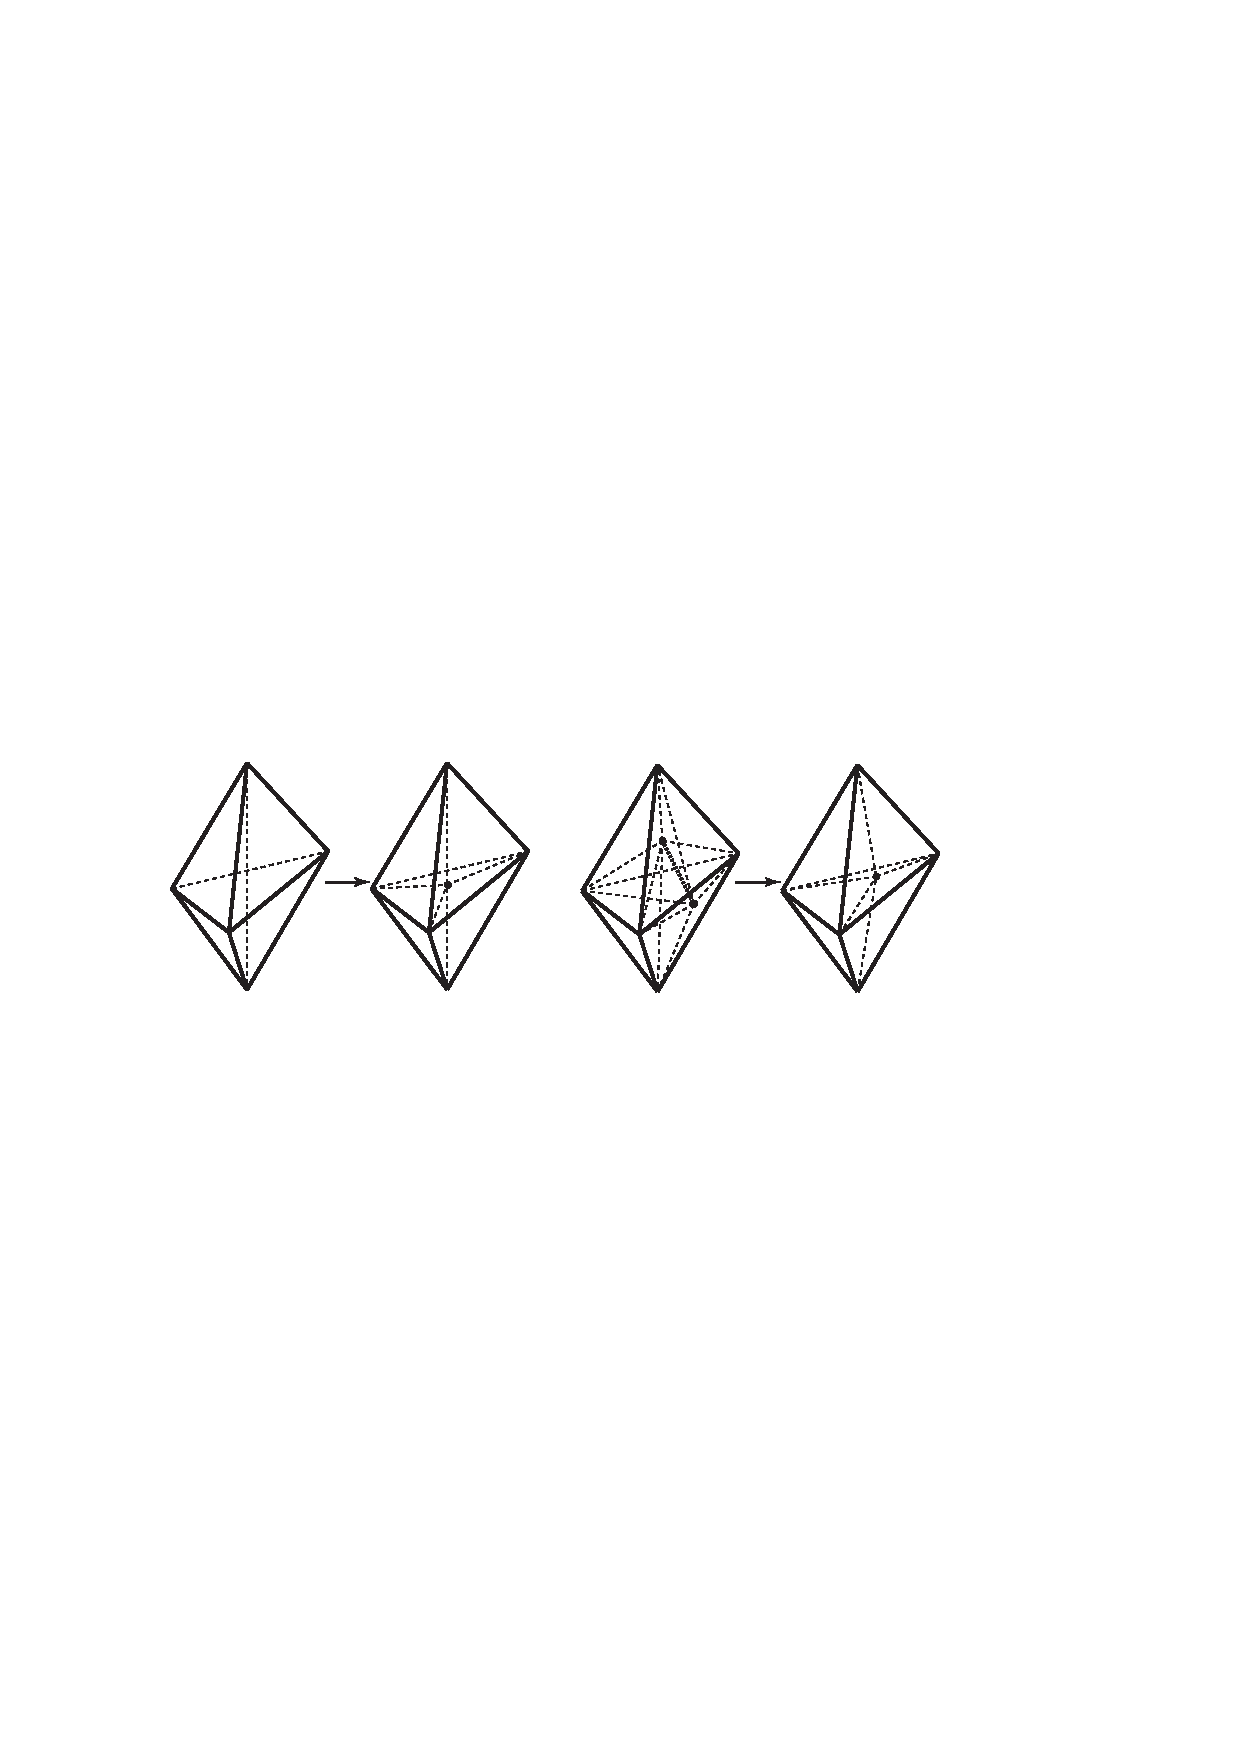
\includegraphics[width=8.0cm]{images/EdgeSplitCollapse}
\caption{Example of the edge split (left) and edge collapse (right)
  operations in 3D. The edge is split at its midpoint and the newly
  created node is then connected to the vertices of the elements
  containing the edge, thus creating additional elements. For edge
  collapse, the elements surrounding the edge are deleted and a node
  placed at the midpoint of the removed edge.}
\label{Fig:EdgeSplit}
\end{figure}
\begin{figure}
\centering
\noindent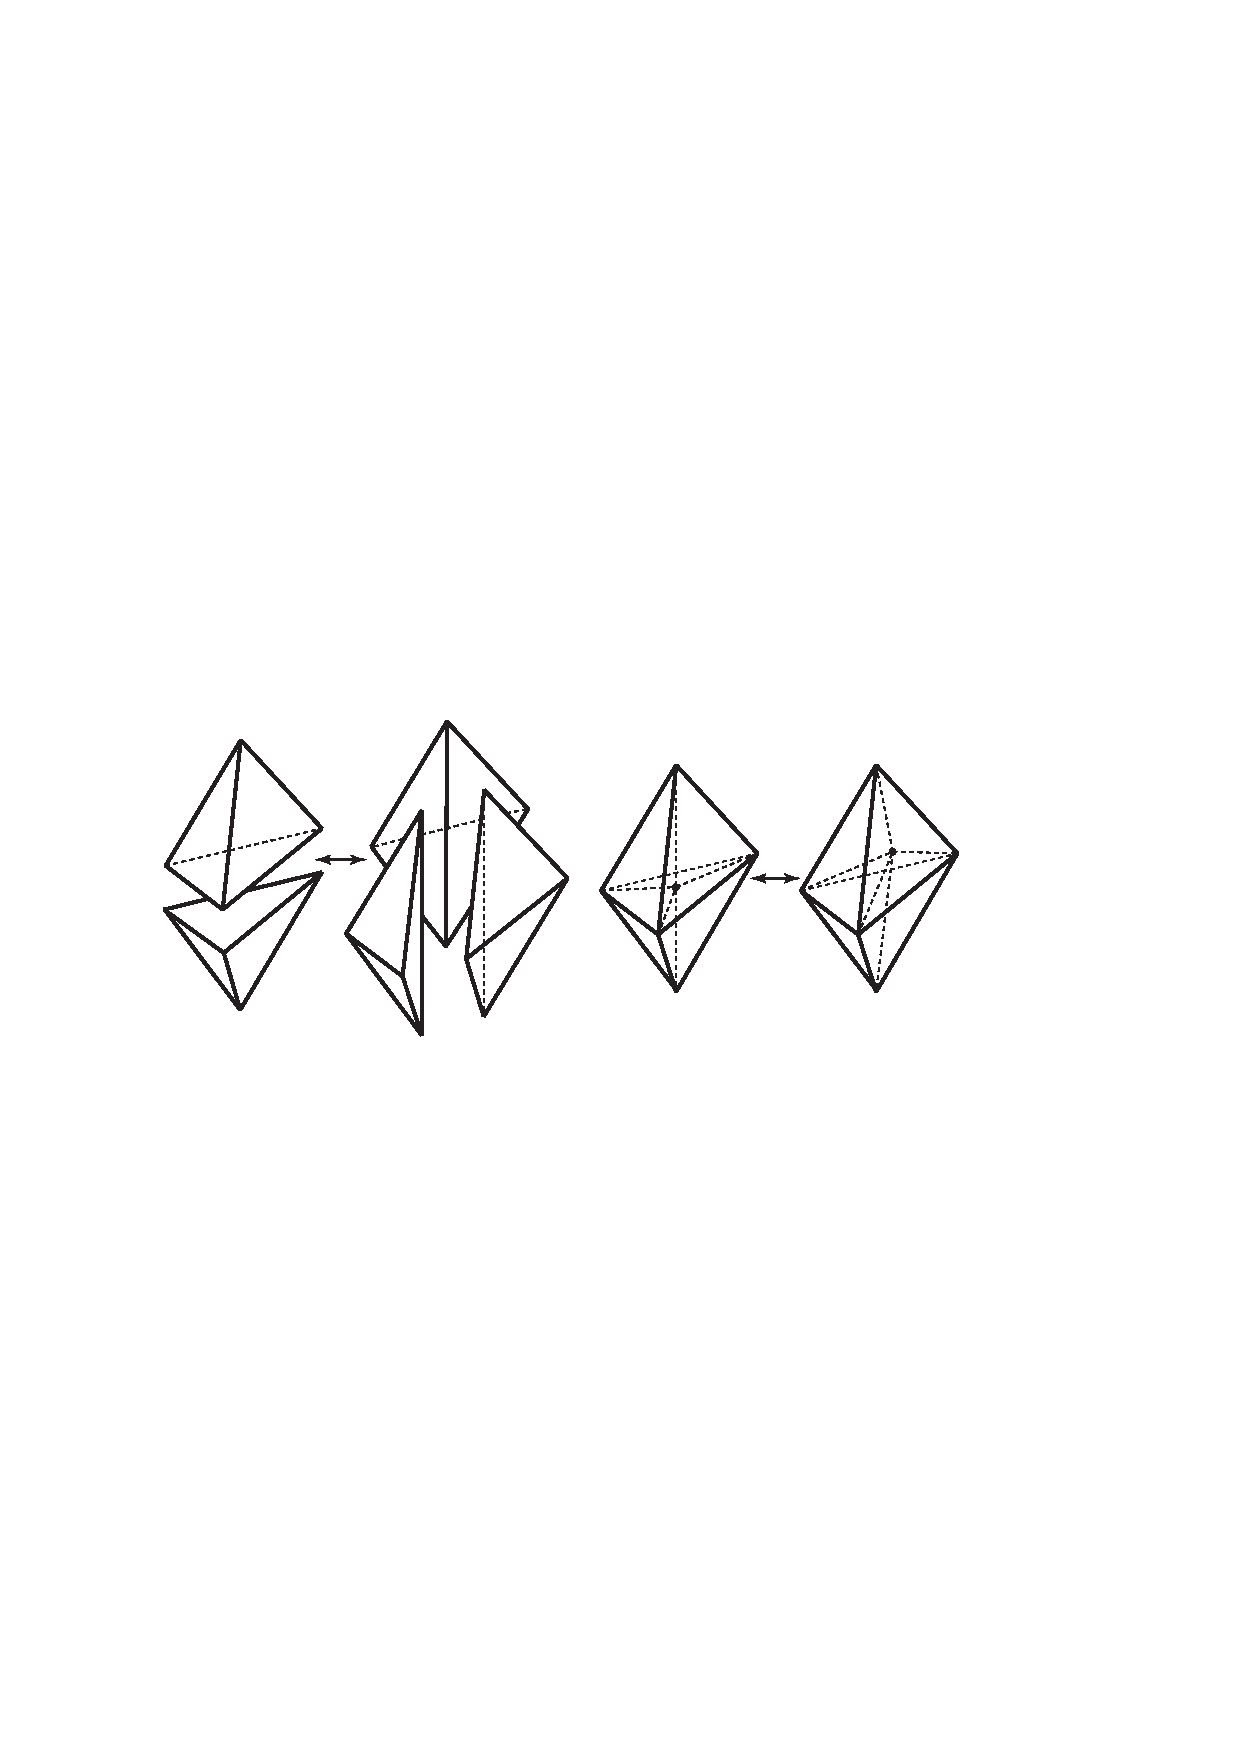
\includegraphics[width=8cm]{images/EdgeFaceNodeMove}
\caption{An example of the face to edge and edge to face swapping
  operation (left) and node movement (right) in 3D.}
\label{Fig:face2edge}
\end{figure}

\begin{figure}
\centering
\noindent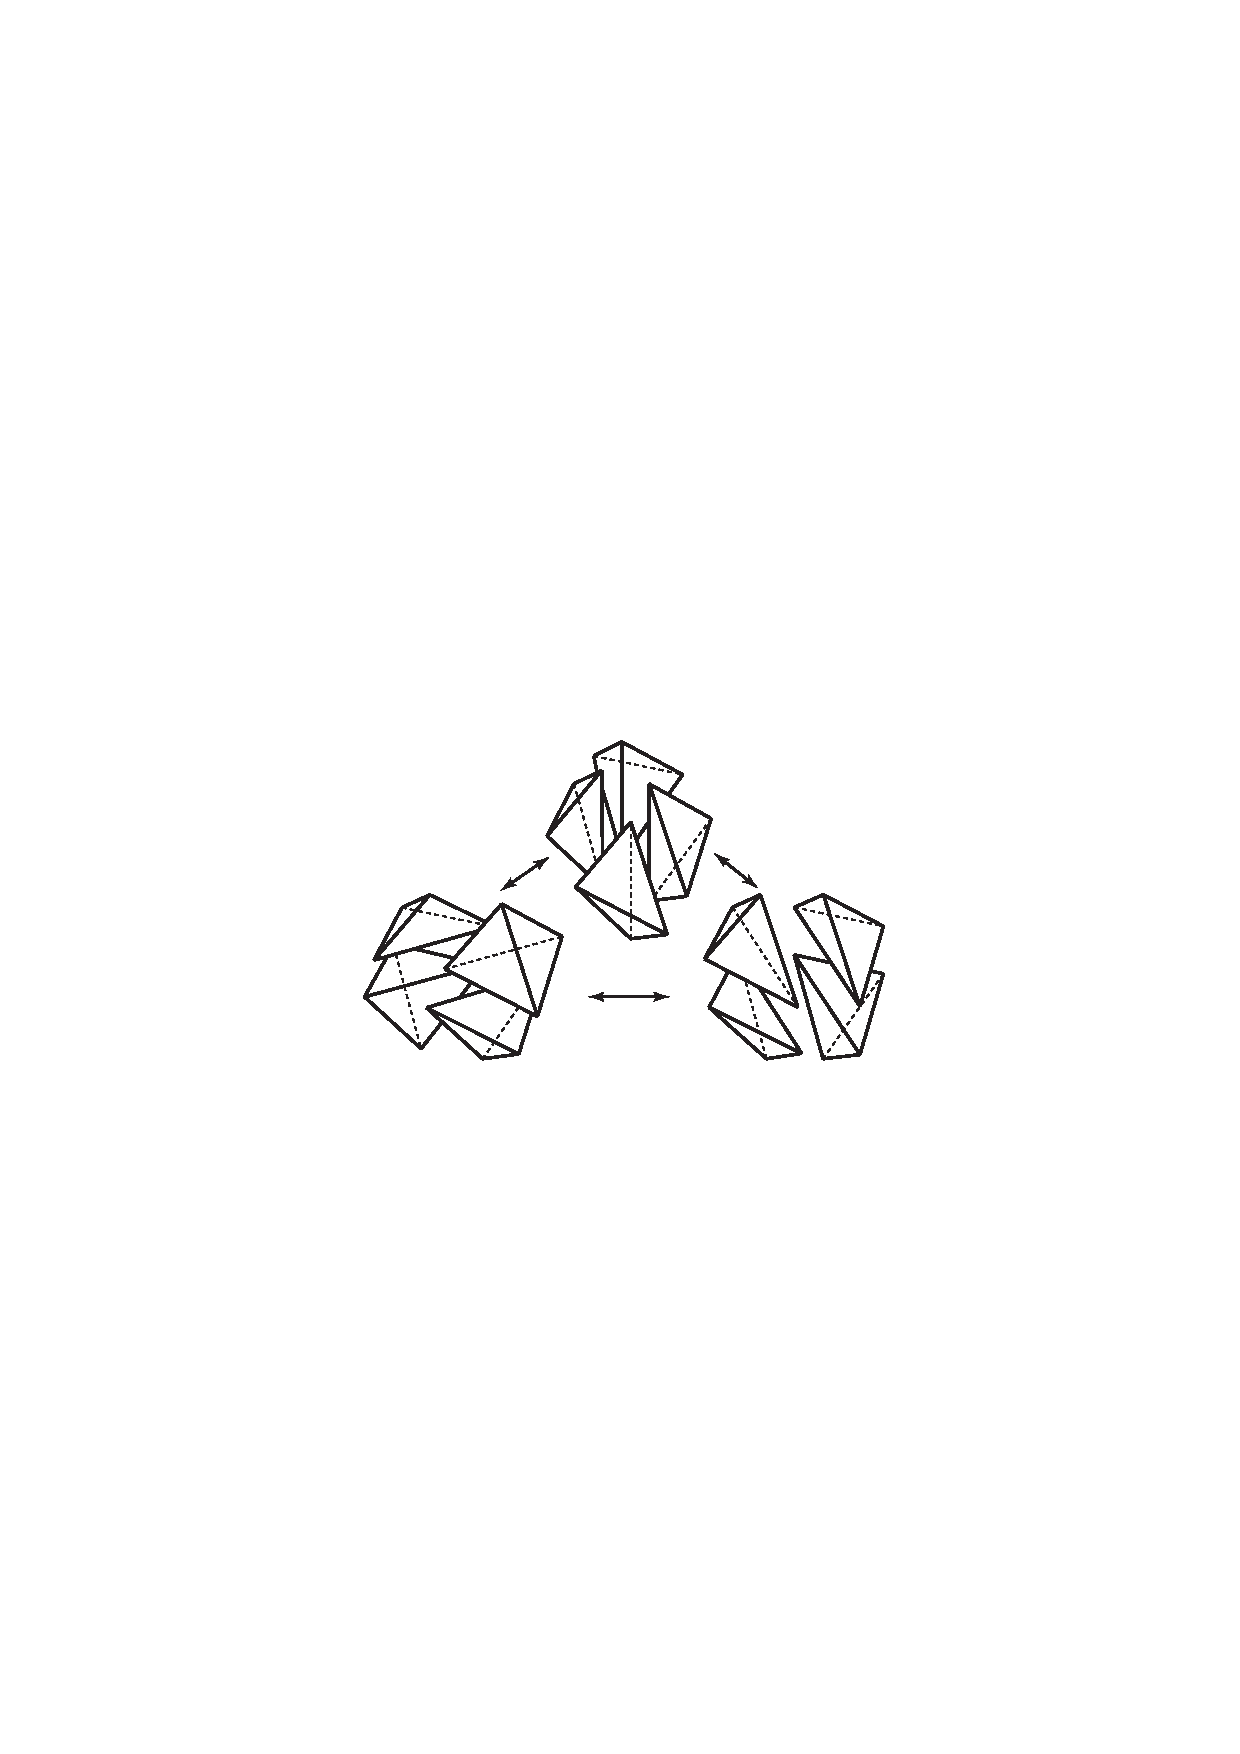
\includegraphics[width=7cm]{images/edge2edge}
\caption{An example of the topological operation of edge to edge
  swapping in 3D.}
\label{Fig:edge2edge}
\end{figure}

Approaches based on these operations are often referred to as mesh
optimisation methods since they involve the definition of some
objective function, usually a norm over the entire mesh of a local
mesh quality estimate. Optimisation of the mesh progresses by
improving the worst elements through a series of elemental
modifications to the mesh in an attempt to minimise the functional and
hence improve the overall quality of the mesh. Dynamic mesh
optimisation is achieved through the construction of metric with which
the objective functional is evaluated and which is itself dependent on
the computed solution fields \citep{simpson1994, buscaglia1997,
  pain2001, piggott2005, power2006}. This allows local anisotropic
features in a solution to be made isotropic in a warped domain through
a coordinate transformation.

\subsection{Mesh optimisation operations}

\begin{figure}
\centering
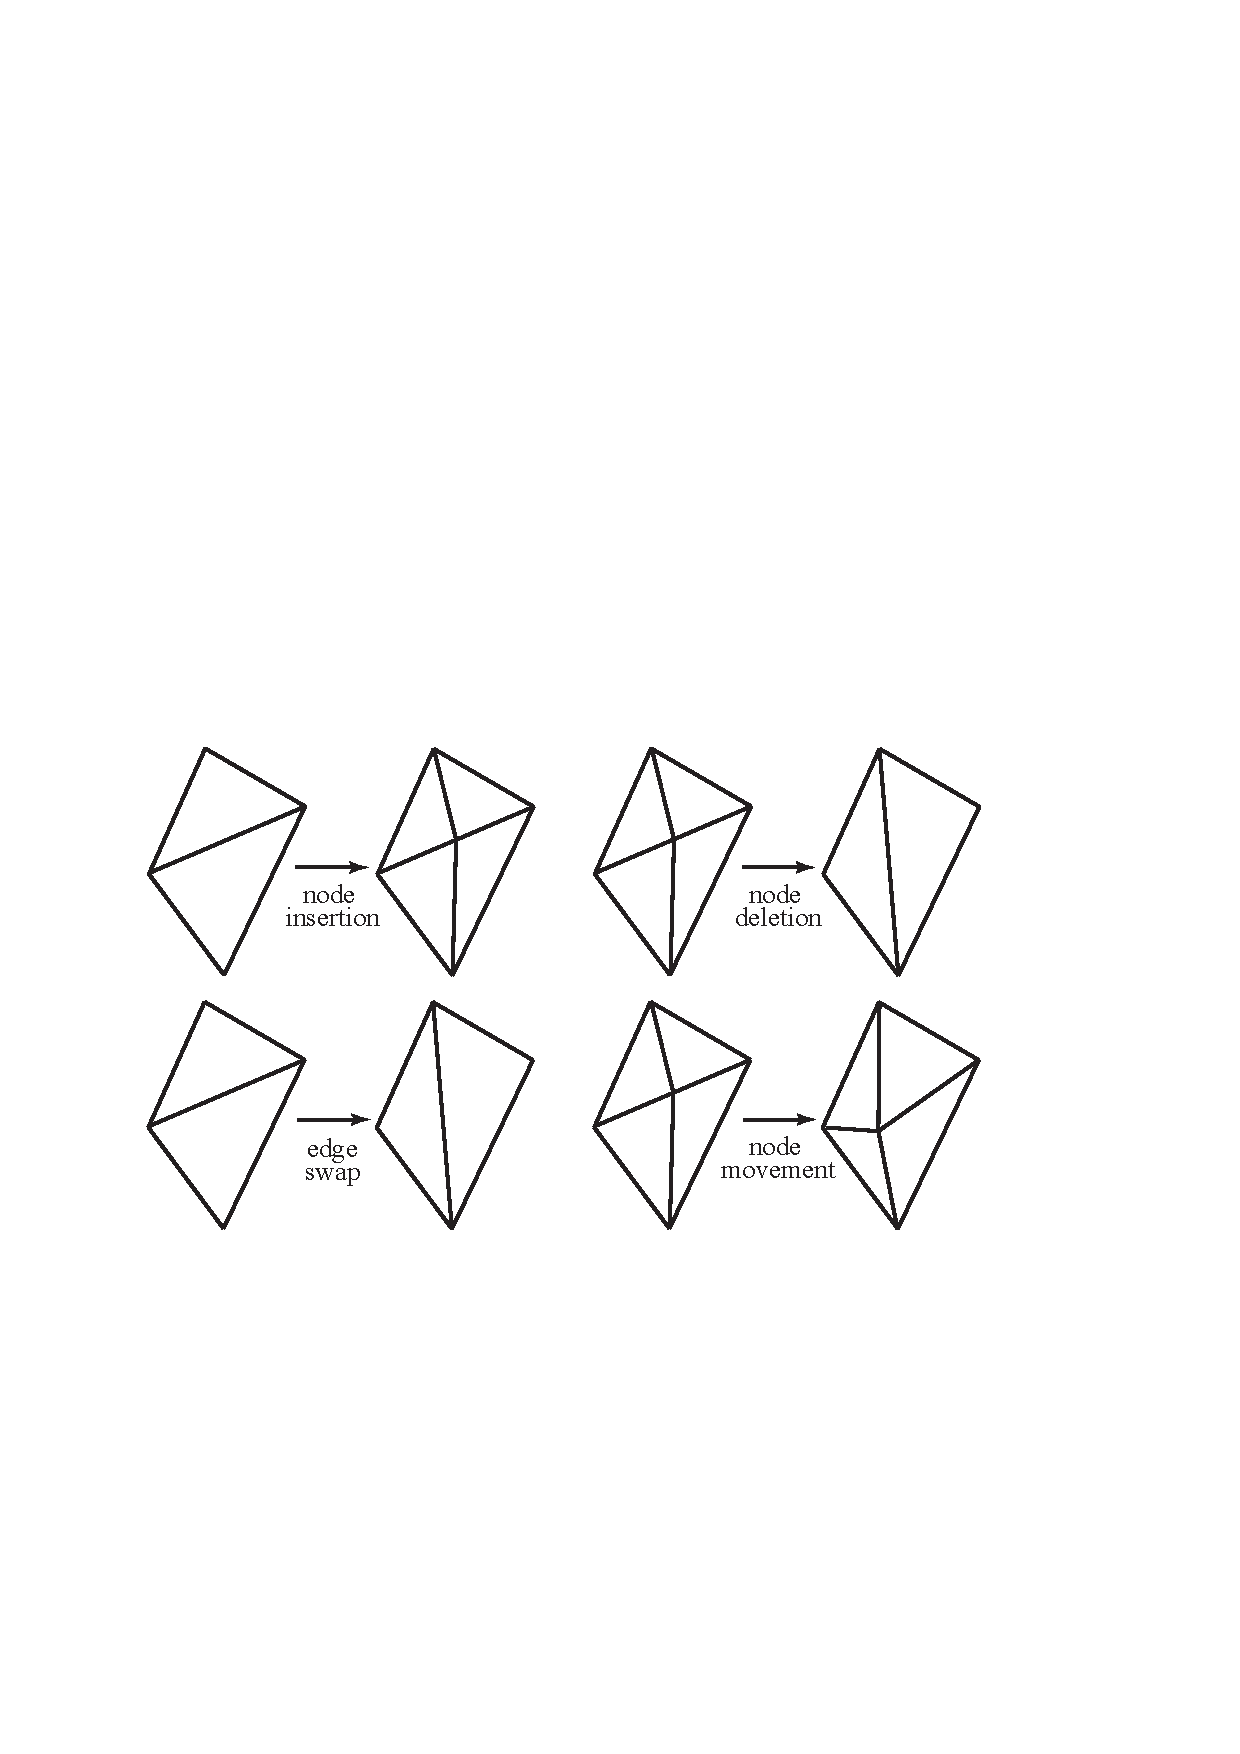
\includegraphics[width=10.0cm]{images/MeshOperations2D.pdf}
\caption{Local element operations used to optimise the mesh in two
  dimensions. Top-left: node insertion or edge split.  Top-right: node
  deletion or edge collapse. Bottom-left: edge swap. Bottom-right:
  node movement.}
\label{Fig:MeshOperations}
\end{figure}

Given an unstructured mesh and information regarding the ideal shape
and sizes of the elements making up the mesh, an optimisation-based
adaptivity algorithm can be formulated via the use of local
topological operations which seeks to improve the quality of elements.

In the examples presented in this work a two-dimensional mesh
optimisation algorithm \citep{agouzal1999,vasilevskii1999adaptive} is used
which employs the following local operations depicted in figure
\ref{Fig:MeshOperations}:
\begin{itemize}
\item Node insertion or edge split -- here a node is inserted on a
  pre-existing edge in the mesh so that the four new elements have
  improved shape/size characteristics than the original two; while the
  location of this new node along the pre-existing edge can be
  optimised, it is common to simply split it at its mid-point.
\item Node deletion or edge collapse -- here the inverse operation is
  performed where an edge in the mesh is collapsed, and consequently a
  node is deleted and two elements removed from the mesh.
\item Edge swap -- here an edge between two elements is removed and
  replaced with the only other possible configuration in two
  dimensions; the number of nodes and elements is preserved through
  the operation, but the edge lengths and elements shapes are
  manipulated.
\item Node movement -- here a node is moved so as to improve the
  quality of all the elements surrounding it; the direction in which
  to move the node can be calculated by considering a discrete
  gradient of the mesh quality functional and performing a line search
  in this direction.
\end{itemize}

The local operations employed in 3D are:
\begin{itemize}
\item{Edge split:} a node is inserted at the centre of an edge and
  surrounding elements created (Fig. \ref{Fig:EdgeSplit}).
\item{Edge collapse:} all elements belonging to the edge are deleted
  and the two nodes of the edge collapsed to its centre (Figure
  \ref{Fig:EdgeSplit}), in cases where one of the nodes is used to
  define the domain geometry the nodes are collapsed to that point, if
  both nodes define some geometrical structure then this operation is
  not permitted.
\item{Edge-face swap:} if two tetrahedra share a common face, and
  provided their combined interior is convex, the face is deleted and
  a new edge introduced between the two nodes not shared thus
  producing three tetrahedra with different alignment
  (Fig. \ref{Fig:face2edge}). The inverse operation where an edge is
  replaced by a face is also allowed.
\item{Edge-edge swap:} $S$ elements are assumed to lie around an edge
  which may be replaced by a different edge resulting in $2S-4$
  elements with different alignment (Fig. \ref{Fig:edge2edge}).
  \cite{freitag1997} found that for increasing $S$ the number of
  transformations that improve the mesh decline dramatically: for this
  reason, this operation is limited to $S\le 4$.
\item{Limited node movement:} the local topology of the mesh is
  preserved but mesh quality is improved by visiting each node and
  moving it to the centroid of all surrounding nodes, \ie\  ensuring
  that when measured in metric space the lengths of all edges attached
  to this node are approximately equal (Fig. \ref{Fig:face2edge}).
\end{itemize}

\subsection{The objective functional}
In order to decide whether the operations described above improve the
quality of the mesh, an objective functional measuring the quality of
the mesh must be defined.  The functional is constructed in order to
gauge mesh quality and whose maximisation is the goal of the
optimization algorithm.

Many measures of element quality have been proposed. In general, for
mesh generation applications Euclidean geometric metrics are
considered \cite{knupp2000achievingI,
  knupp2000achievingII}. However, these metrics do not take into
account characteristics of the solution. Therefore, other measures of
element quality have been proposed which do take into consideration both
the shape and size of the elements required for controlling solution
errors.

In the work described here, we use the element quality measure for 2D
simplexes proposed by Vasilevskii \etal\
\cite{vasilevskii1999adaptive}:
\begin{equation}\label{eqn:quality2D}
q^M(\triangle) = \underbrace{12\sqrt{3}\frac{|\triangle|_M}{|\partial\triangle|_M^2}}_{I} \underbrace{F\left(\frac{|\partial\triangle|_M}{3}\right)}_{II},
\end{equation}
where $|\triangle|_M$ is the area of element $\triangle$ and
$|\partial\triangle|_M$ is its perimeter as measured with respect to
the non-Euclidean metric $M$ as evaluated at the element's centre. The
first factor ($I$) is used to control the shape of element
$\triangle$. For an equilateral triangle with sides of length $l$,
$|\triangle| = l^2\sqrt{3}/4$ and $|\partial\triangle| = 3l$; and so
$I=1$. For non-equilateral triangles, $I<1$. The second factor ($II$)
controls the size of element $\triangle$. The function $F$ is smooth
and defined as:
\begin{equation}
F(x) = \left(\min(x, 1/x)(2 - \min(x, 1/x))\right)^3,
\end{equation}
which has a single maximum of
unity with $x=1$ and decreases smoothly away from this with
$F(0)=F(\infty)=0$. Therefore, $II=1$ when the sum of the lengths of the
edges of $\triangle$ is equal to $3$, \eg\ an equilateral triangle with
sides of unit length, and $II<1$ otherwise. Hence, taken together, the
two factors making up $Q$ yield a maximum value of unity for an
equilateral triangle with edges of unit length, and $Q$ is less than
one otherwise. 

We use an analogous measure of element quality proposed by Agouzal
\etal\ for 3D simplexes \cite{agouzal1999}.

Mesh optimization is now performed on the mesh via a sequence of local
topological and geometrical operations \citep{pain2001,freitag1997}
which seek to efficiently minimise the objective functional. The algorithm
proceeds in a Gauss-Seidel iterative manner. Each of the elements are
visited in turn and the local mesh structure of the element and its
neighbours altered via the operations described above. If an operation
is found to improve the mesh quality as measured by the functional,
it is retained.

\subsection{Error measures and metrics}
Mesh adaptivity requires an error measure to guide it. Hierarchical
mesh refinement algorithms are typically guided by error measures
which associate a scalar to each element, measuring the contribution
of that element to the error in some quantity of interest. Anisotropic
mesh adaptivity \citep{simpson1994, buscaglia1997, pain2001, li2005,
  frey2005} requires directional information at each point in the
domain, and thus is typically guided by an error metric, a tensor
field defined over the domain.  Anisotropic mesh adaptivity exploits
any anisotropic features of the solution fields to be represented,
increasing the computational efficiency of the simulation by
minimising the number of nodes and elements required to adequately
represent the solution fields.

In one dimension, the interpolation error over a linear element is
bounded by the second derivative of the function being
interpolated. This result carries over to higher dimensions, with the
second derivative replaced by the Hessian of the function being
interpolated, the tensor field of second partial derivatives
\citep{frey2005}. The Hessian describes the curvature of the solution
at each point in every direction; using the Hessian for the error
metric to guide anisotropic mesh adaptivity places resolution where
the solution field curves. For elliptic problems, C\'ea's lemma shows
us that the interpolation error bounds the discretisation error in the
energy norm; in practice, minimising the interpolation error in this
manner has been found to be highly effective at controlling the
discretisation error, even for non-elliptic problems.

In the previous sections mesh optimisation operations and an objective
functional have been introduced.  These can be used together to
formulate an optimisation approach to deliver optimally shaped
elements within a given domain. The element quality depends upon the
area and edge lengths of the element and these scalars were defined in
terms of a metric $M$. Assuming that this is the standard Euclidean
metric then this procedure would seek to deliver uniformly sized
equilateral triangles in the domain. To turn this procedure into one
which delivers variable anisotropic resolution a non-Euclidean metric
$M({\bf x})$ can be used. Given element $\triangle$ one may assume,
both for simplicity of explanation and also numerical implementation,
that $M$ is constant over $\triangle$. In this case
\begin{equation*}
|\triangle|_M = \sqrt{\textrm{det}(M)}|\triangle|_E,\quad
|\partial \triangle|_M = \sum_{i=1}^{3} ||\partial \pmb{e}_i||_M = \sum_{i=1}^{3} \sqrt{\pmb{e}_i^T M {\bf e}_i},
\end{equation*}
where $|\triangle|_E$ is the area of element $\triangle$ in the
standard Euclidean metric, $\pmb{e}_i$ is the vector representing the
$i$-th edge of element $\triangle$ and $||\partial \pmb{e}_i||_M$ is
its length with respect to the metric $M$.

The choice of $M$ is critical in achieving an adapted mesh that in
some heuristic sense is optimal for given solution characteristics.
Interpolation error estimates form an excellent starting point for the
construction of a suitable metric $M$.  In one dimension, the linear
interpolation error of a smooth function is bounded by the product of
the second derivative of the function being interpolated and the size
of the region being considered. For example, for a finite element
approximation this would be the size of the element the
piecewise-linear interpolant is defined over.  In higher dimensions a
similar result holds with the second derivative replaced by the
Hessian of the function being interpolated, the tensor field of second
partial derivatives \citep{dazevedo1991,george1998,frey2005}. The
Hessian describes the curvature of the solution at each point in every
direction; using the Hessian as a basis for the metric $M$ results in
enhanced resolution where the solution field has high curvature. For
elliptic problems, C\'ea's lemma shows us that the interpolation error
bounds the discretisation error in the energy norm; in practice,
minimising the interpolation error in this manner has been found to be
highly effective at controlling the discretisation error, even for
non-elliptic problems.

For a mesh of triangles in 2D, assume a sufficiently smooth function
$u\equiv u(\pmb{x})$ is approximated by its piecewise-linear Lagrange
interpolant $\Pi_h u$ on element $\triangle$. The interpolation error
on element $\triangle$ satisfies
\begin{equation}
\epsilon_u\equiv ||{u} - \Pi_h{u}||_{\infty,\triangle}
\le c\cdot
\max_{\pmb{x}\in \triangle}\max_{\pmb{v}\subset \triangle} \pmb{v}^T |H| \pmb{v}
\le c \cdot\max_{\pmb{e}\in E_{\triangle}}\pmb{e}^T |\bar{H}| \pmb{e},
\label{highDint}
\end{equation}
where $c$ is a constant independent of the mesh, $\pmb{v}$ is a vector
in $\triangle$, $E_{\triangle}$ is the set of edges of $\triangle$,
$||\cdot||_{\infty,\triangle}$ is the infinity norm over $\triangle$,
and $\bar{H}$ is an element-valued Hessian defined such that
(\ref{highDint}) holds \cite{frey2005}. $|H|$ denotes the positive
definite metric formed by taking the absolute value of the eigenvalues
of ${H}$ and reflects the fact that it is the magnitude of the
curvature that is of interest, rather than the sign of the curvature.

Alternatively, the square of the eigenvalues can be used; this
optimises for the gradient error \citep{dazevedo1991, shewchuk2002}
and leads to elements with larger aspect ratios.

For a target, possibly spatially and temporally varying, interpolation
error, $\epsilon_u$, a metric $M$ is defined such that, assuming
$c=1$, an element edge length is unity with respect to $M$ if it has
the desired interpolation error, \ie\
\begin{equation}
  M = \frac{1}{\epsilon_u} {|\bar{H}|}.
  \label{eqn:ME}
\end{equation}
Construction of an adapted mesh which equidistributes the
interpolation error throughout the domain can be seen from
(\ref{highDint}) to be equivalent to the construction of a uniform
mesh of equilateral tetrahedra, \ie\ all element edge lengths are
unity with respect to $M$. It is the element quality that defines how
close to this requirement of equidistribution each element is.  For
other approaches to the construction of error metrics see
\cite{micheletti2005,power2006,bernard2007}.

A symmetric positive-definite metric tensor $M$ may be decomposed as
\begin{equation*}
M = Q \Lambda Q^T,
\end{equation*}
where $\Lambda$ is the diagonal matrix consisting of the eigenvalues
of $M$ (the principal curvatures of the solution field for $M=H$) and
$Q$ is an ortho-normal matrix of eigenvectors ${Q}^i$. $Q$ may be
interpreted geometrically as a rotation and $\Lambda$ a rescaling.
The eigenvalue $\lambda^i$ encodes the desired edge length in the
direction ${Q}^i$ as
\begin{equation*}
h^i = 1 / \sqrt{{\lambda}^i},
\end{equation*}
\ie\ anisotropic as well as inhomogeneous resolution results from a
mesh that respects the metric $M$. Note that the transformation
${\bmv}=Q\sqrt{|\Lambda|}^{-1}\tilde{\bmv}$ may be used to transform a
uniform isotropic element in a computational space into an adapted
anisotropic element in the physical domain achieving the desired
interpolation error everywhere,
Fig. \ref{Fig:Transformed_Elements}. This can be seen from the
decomposition of $M$ above and
\begin{equation*}
1={\bmv}^T  M {\bmv} = (\sqrt{|\Lambda|}Q^T\bmv)^T(\sqrt{|\Lambda|}Q^T\bmv)=\tilde{\bmv}^T\tilde{\bmv}.
\end{equation*}

\begin{figure}
\centering
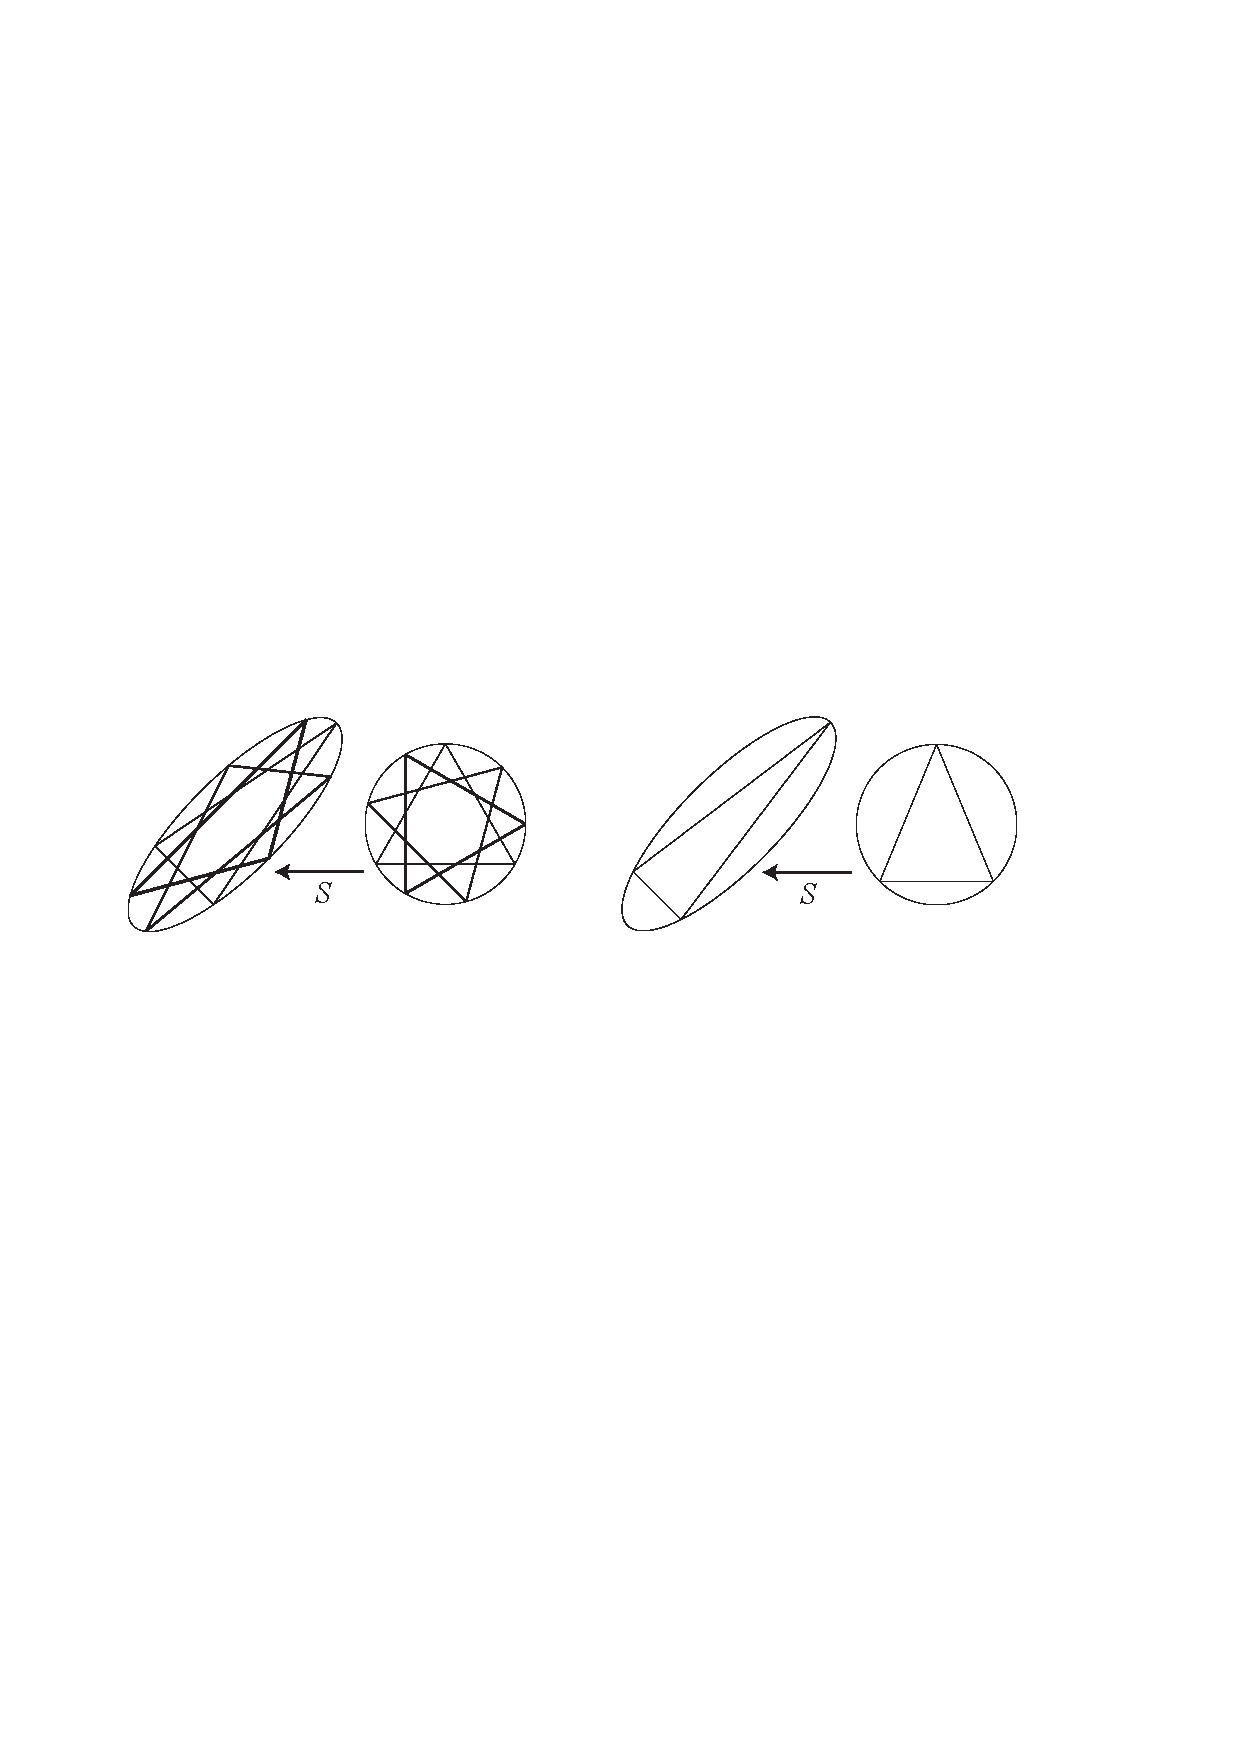
\includegraphics[width=12cm]{images/Transformed_Elements.pdf}
\caption{Mapping of triangular elements between physical and metric
  space.  Left: those elements in physical space which are of the
  appropriate size and aspect ratio, and which are of maximal area,
  can be shown to map to the unit equilateral triangle in metric space
  under the transformation $S=Q\sqrt{|\Lambda|}^{-1}$.  Right: an
  element which does not maximise area and consequently transforms to
  a non-equilateral triangle in metric space.}
\label{Fig:Transformed_Elements}
\end{figure}

\cite{george1998} (pg. 350) point out that use of a global error norm
can in fact alter the error analysis by enhancing the accuracy of
regions with high solution magnitude where changes are clearer than
those regions of low magnitude. To overcome this, it is possible to
use a {\it relative error},
\begin{equation*}\label{eqn:relative_error_3D}
  \epsilon_r=\frac{\pmb{v}^T \pmb{H} \pmb{v}}{\max(\|\psi\|, \psi_{min})},
\end{equation*}
giving a new metric tensor,
\begin{equation*}\label{eqn:relative_metric}
  \pmb{M}_r = \frac{\vert\pmb{H}\vert}{\epsilon_r\max(\|\psi\|, \psi_{min})},
\end{equation*}
for some positive $\psi_{min}$. $\psi_{min}$ is required to be some
number greater than zero to avoid division by zero, but it can also be
used to suppress curvature values associated with small values of
$\psi$ which may be considered spurious. It is important to note that
while in (\ref{eqn:ME}), the interpolation error, $\epsilon_g$, has
the same dimensions as the solution field, the relative interpolation
error, $\epsilon_r$, is dimensionless and $100\epsilon_r$ is the
percentage error.


\subsection{Combining multiple fields and bounding aspect ratio and edge lengths}

For complex problems one will wish to simultaneously adapt the mesh
for several solution fields. The approach taken here is to use a
single mesh to represent all fields and hence typically a compromise
needs to made. Often this compromise will not be substantial since in
many problems regions and directions of high curvature are common
between solution fields. For oceanographic problems the base set of
fields we would want to adapt to are the components of velocity,
temperature and salinity. Metric fields are constructed for each with
their own interpolation errors. A superposition procedure is then
undertaken so that a single metric results which respects the edge
length and requirements of each individual metric. The procedure is
shown graphically in figure \ref{Fig:MergedMetrics} and follows
\cite{pain2001}, see also \cite{castrodiaz1997,george1998}.

\begin{figure}
\centering
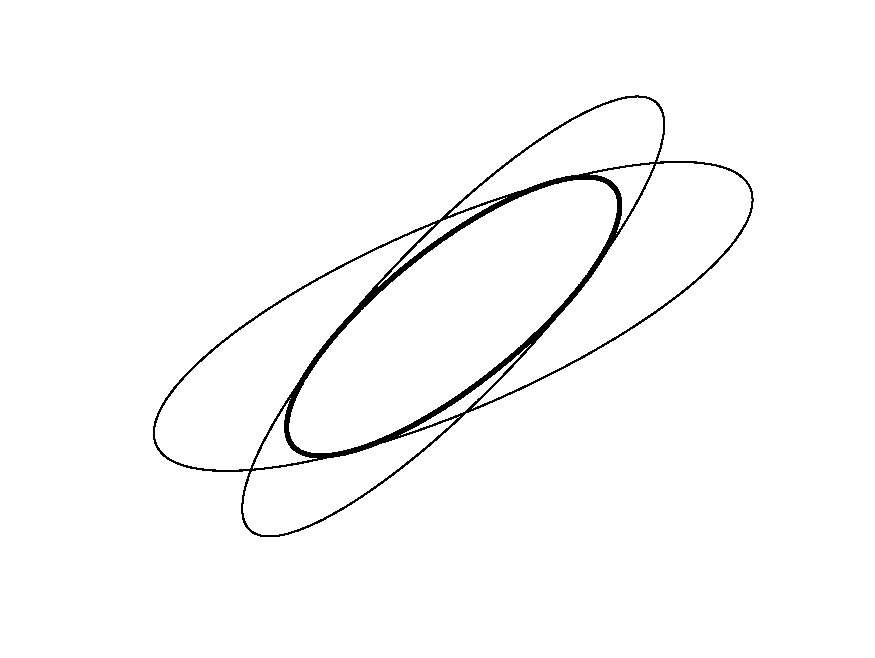
\includegraphics[width=5cm]{images/MergedMetrics.pdf}
\caption{The superposition of two metrics to yield a third which
  respects the edge-length requirements of both.  The metrics are
  shown here graphically as ellipses. The two original metrics are
  shown in faint lines, the new superimposed metric, or maximal inner
  ellipse, is represented by the bold line}
\label{Fig:MergedMetrics}
\end{figure}

In addition, it is sometimes advantageous to modify the metric to
impose maximum and minimum element sizes on the mesh: for example, to
stop the optimisation procedure from attempting to produce elements
larger than the solution domain, or smaller than a certain scale which
the user deems to be unimportant, or which they wish to use
subgrid-scale models to represent. Also, for problems which have known
high aspect ratio dynamics or domains it can be necessary to impose
these maximum and minimum constraints directionally. The approach
taken to achieve this here is to construct extra metrics describing
maximum and minimum edge lengths. For example, assuming the user
wished to limit the maximum element sizes in the x and y directions to
be $h_{x,\textrm{max}}$ and $h_{y,\textrm{max}}$ respectively, then
the metric $M_{\textrm{max}} =
\textrm{diag}((h_{x,\textrm{max}})^{-1/2},(h_{y,\textrm{max}})^{-1/2})$,
could be superimposed.  For the minimum edge length metric the $\max$
operator must be replaced with a $\min$ operator. More general
directions for the maximum and minimum edge lengths can be introduced
through the use of the rotation matrix $Q$.

To bound the aspect ratio of elements in physical space a limit on the
ratio of eigenvalues may also be performed. For example, to limit the
aspect ratio of elements to be below $a$ the eigenvalues of the metric
can be modified as follows:
\begin{equation*}
{\lambda}'_j=\max\left\{\tilde{\lambda}_j,\frac{1}{a^2}\max_{i=1,2}\tilde{\lambda}_i\right\},\;\; j=1,2,
\end{equation*}
\ie\ this operation seeks to limit the minimum eigenvalue, and hence
the maximum edge length in an element.  It thus achieves a maximum
bound on aspect ratio without compromising the interpolation error
achieved over that element.

\subsection{Hessian recovery}
We recall the definition of the Hessian.  Given a function
$u=u(\pmb{x}) \in C^2(\Omega)$ we define the Hessian $\pmb{H}$ as the
tensor of second-order partial derivatives, where its matrix
contributions are
\begin{equation} \label{eqn:hessian}
  \pmb{H}_{ij} = \frac{\partial^2u}{\partial x_i \partial x_j}.
\end{equation}
For $C^2$ functions, the Hessian is symmetric.

In practice only the discrete interpolant is available, not
an analytical formula for the function being interpolated. Thus it is
necessary to recover a discrete approximation to the true Hessian, and
use this to guide anisotropic adaptivity. Typically, we wish to obtain
a piecewise linear approximation to the Hessian.

Different recovery schemes such as quadratic fitting
\citep{vallet2007}, superconvergent patch recovery
\citep{zienkiewicz1992}, integration by parts \citep{buscaglia1997}
and double lumped $L^2$ projection \citep{pain2001} have been
suggested. In this work, we use the double lumped $L^2$ projection.
We employ a weak finite element formulation for the Hessian as
\begin{equation*}
\pmb{H}^k_{ij} = \frac{1}{M^{k}_L} \ \int_\Omega \ \phi_k \frac{\partial q_i}{\partial x_j} dV,
\end{equation*}
where $q_i$ is a piecewise linear projection of the first derivative given by
\begin{equation} \label{var_first_derivative}
q_i = \frac{1}{M^{k}_L} \ \int_\Omega \ \phi_k \frac{\partial u}{\partial x_i} dV.
\end{equation}
The off-diagonal entries are then averaged to enforce symmetry of the computed
Hessian.

\subsection{Load balanced parallelisation}
The principal challenges associated with the parallelisation of a
computational model based on adaptive meshes are: consistency of
shared node and element information between subdomains; minimisation
of communication overhead costs; and dynamic load-balancing. Mesh data
consistency refers to the requirement that all processors that have
information regarding particular mesh entities (\ie\ nodes, elements,
auxiliary), have that information correctly updated as part of the
mesh adaptivity process, and that the complete mesh remains conformal
after the application of mesh optimisation (\ie\ no hanging nodes are
allowed). After mesh optimisation has been performed, load-imbalances
are to be expected as nodes and elements are in general added and
deleted according to solution requirements, thus the distribution of
work may vary across subdomains. The obvious exception to this is the
r-method as the number of nodes and mesh connectivity does not change
--- clearly an attractive property for parallel computation.  There is
a great deal of interest in dynamic load-balancing and cost modelling
for parallel mesh optimisation --- deciding when the mesh needs to be
repartitioned among the processors involved in the computation,
methods for calculating such a repartitioning and efficiently
realising the new partitioning through data migration (also referred
to as data remapping).

When mesh optimisation methods are applied in parallel, one must
consider what happens to mesh entities which are shared between
processes as optimisation uses Gauss-Seidel type sweeps of the entire
mesh, and the mesh must of course be conformal throughout the
processes. A method based on maximal independent sets is used to
accomplish this \citep{jones1997, freitag1999b, freitag1999}. By only
allowing mesh entities of the same colour to be updated within a
parallel mesh optimisation iteration, it can be ensured that the
shared mesh entities are not updated simultaneously on different
partitions. In this context, a node of the graph to be coloured is
defined by the set of nodes and elements which would be modified by a
local operation, while the edges of the graph is a superposition of
the mesh node and element adjacency lists --- this is the so called
task graph which of course changes for different elemental
operation. The task graph defines the mesh entities that must be
updated when an elemental operation is performed and thus defines the
data that must be synchronised at the end of an adaptive step. Broadly
speaking, the parallel mesh adaptivity method involves sweeping
through graph entities of the same colour in sequence, and then
synchronising changes after each colour has been processed
\citep{freitag1999}.

\subsection{Mesh-to-mesh interpolation}
By changing the mesh, an adaptive algorithm also changes
the function space associated with the mesh. Therefore, adaptivity
necessitates an interpolation step between the previous and adapted
meshes so that the simulation may be timestepped forward.

The natural algorithm for interpolating from a donor mesh to a target
mesh, called consistent interpolation, is the interpolation derived
from the solution values of the donor mesh. For each node $n_{\cal{T}}
\in \cal{N}_{\cal{T}}$ in the target mesh $\cal{T}$, a containing
element $K_{\cal{D}}$ is identified in the donor mesh $\cal{D}$, and
the solution $q(\pmb{x})$ is evaluated at the physical location of the
target node $n_{\cal{T}}$. Such an element $K_{\cal{D}}$ may be
identified by an advancing front algorithm \citep{lohner1995} or by an
R-tree spatial indexing algorithm \citep{guttman1984}.

This algorithm is cheap to implement and is bounded for piecewise
linear basis functions. It is not conservative: the integral of the
interpolant on the target mesh will not in general be the same as the
integral of the field on the donor mesh. The method can be diffusive:
unless nodes in the new mesh exist at the maxima and minima of the
function on the old mesh, the maxima and minima may be lost. The
algorithm is also not defined for discontinuous meshes.

An alternative is to project from the donor mesh to the target mesh;
that is, to find the element of the target function space which is
closest in the $L_2$ norm to the function being interpolated. This is
referred to as Galerkin projection \citep{george1998}. Doing this
between arbitrarily unrelated unstructured meshes requires the
construction of a supermesh of the target and donor meshes; this may
be thought of as the mesh of intersections of the elements of the
target and donor meshes
\citep{farrell2009a,farrell2011conservative}. Galerkin projection is
conservative, minimally diffusive, and can be made bounded, but is
more expensive than consistent interpolation.
